\section{Conceptos básicos del \SM}
\label{cap:sm}

\subsection{Las partículas elementales y sus interacciones}

De acuerdo al SM toda la materia esta compuesta por un número peque\~no de
partículas fundamentales, fermiones, de espín $\frac{1}{2}$ que se dividen en
dos tipos: <<\emph{quarks}>> y <<leptones>> (ver \cref{tab:fermions}). Hasta el
momento, ningún experimento ha podido encontrar evidencia de que estos fermiones
tengan una subestructura interna. Los \emph{quarks} y leptones además están divididos
en tres generaciones o familias, ordenadas según su masa. Las partículas de las
generaciones más altas tienen mayor masa y son inestables, decayendo en
partículas de generaciones más bajas. Es por este motivo que la materia
ordinaria está formada por las partículas estables de la primera generación.

\begin{table}[!h]
  \centering

  \caption{Partículas elementales de materia del SM, incluyendo las
    tres generaciones, ordenadas según su masa. En la
    segunda y tercer columna se encuentra la masa \cite{PDG} y la carga
    eléctrica, respectivamente. En el caso de los neutrinos solo existen cotas
    superiores de su masa.}
  \label{tab:fermions}.

  \begin{tabularx}{\textwidth}{Cx{0.6cm}x{0.6cm}x{0.6cm}CCCC}
    \hline
    & \multicolumn{3}{c}{Partícula} & \multicolumn{3}{c}{Masa} & Carga Eléctrica \\

    \hline
    \multirow{2}{*}{Leptones}
    & e & $\mu$ &  $\tau$ & 511 \kev & 105.7 \mev & 1768 \mev & -1  \\
    & $\nu_e$ & $\nu_\mu$ & $\nu_\tau$ & $<2.2 \eV$ & $< 0.17 \mev$ & $<15.5 \mev$ & 0 \\
    \hline
    \multirow{2}{*}{\emph{Quarks}}
    & $u$ & $c$ & $t$ & 2.4 \mev & 1.27 \gev & 171.2 \gev & $\frac{2}{3}$ \\
    & $d$ & $s$ & $b$ & 4.8 \mev & 104 \mev & 4.2 \gev & -$\frac{1}{3}$ \\
    \hline
  \end{tabularx}

\end{table}

La distintas interacciones entre \emph{quarks} y leptones son descriptas en el SM en
términos del intercambio de partículas entre estos. Estas partículas de
intercambio son los <<bosones de \emph{gauge}>>, y tienen espín igual a 1 (ver
\cref{tab:bosons}). Existen cuatro tipos de interacciones fundamentales. La
interacción fuerte es la responsable de mantener los quarks formando los
protones, neutrones y hadrones en general, y es mediada por partículas no
masivas llamadas gluones. Las interacciones electromagnéticas son las
responsables de los fenómenos extra nucleares, como por ejemplo las fuerzas
intermoleculares en líquidos y sólidos. Estas interacciones están mediadas por
el intercambio de fotones no masivos. La interacción débil es la responsable de
los procesos de desintegración de núcleos y partículas, y sus mediadores son los
bosones $Z^0$ y $W^\pm$, con masas del orden de 100 veces la masa del protón.
Por último existe una interacción que actúa entre todo tipo de partículas, la
interacción gravitatoria. Actualmente no existe ninguna teoría cuántica completa
que explique esta interacción fundamental, aunque hay varias teorías propuestas
que postulan la existencia de una partícula de espín 2 mediadora de la gravedad,
denominada gravitón. En la escala de los experimentos de partículas, la
gravitatoria es la interacción más débil de todas las interacciones
fundamentales, aunque es la dominante en la escala del universo, y será
despreciada en lo que sigue.

Los leptones interactúan de forma débil y electromagnética en el caso de ser
cargados, o solo débilmente si son neutros. En contraste, los \emph{quarks} interactúan
además de débil y electromagnéticamente, por medio de la interacción fuerte.
Esta es la distinción fundamental entre \emph{quarks} y leptones.

Adicionalmente, por cada partícula en el SM, existe una antipartícula asociada,
con todos sus números cuánticos no nulos opuestos. Los bosones de \emph{gauge} neutros
constituyen su propia antipartícula.


\begin{table}[!htb]
  \centering

  \caption{Bosones de \emph{gauge} mediadores de las diferentes interacciones
    fundamentales incluidas en el SM, junto con su masa \cite{PDG} y carga
    eléctrica. }
  \label{tab:bosons}

  \begin{tabularx}{\textwidth}{CCCC}
    \hline
    Fuerza & Partícula & Masa & Carga Eléctrica \\
    \hline
    \multirow{2}{*}{Débil}  &   $W^\pm$ & $80.385 \pm 0.015$ \gev  & $\pm1$ \\
                            &   $Z^0$   & $91.1876 \pm 0.0021$ \gev  & 0 \\
    \hline
    Electromagnética & $\gamma$ & 0 & 0 \\
    \hline
    Fuerte & $g$ & 0 & 0 \\
    \hline
  \end{tabularx}

\end{table}


Formalmente, el {\SM} es una teoría cuántica de campos renormalizable que provee
una descripción de los campos de las partículas elementales, y las interacciones
fuerte, débil y electromagnética. Estas interacciones surgen del requerimiento
de que la teoría sea invariante bajo transformaciones de \emph{gauge} locales del grupo
de simetría:

\begin{equation}
  \text{SU}(3)_\text{C} \times \text{SU}(2)_\text{L} \times \text{U}(1)_\text{Y}
\end{equation}
%
El subgrupo $\text{SU}(2)_\text{L} \times \text{U}(1)_\text{Y}$ representa el sector
electrodébil, es decir, la electrodinámica cuántica (QED) más las interacciones
débiles, donde L\footnote{L indica que $\text{SU}(2)_\text{L}$ actúa solo sobre los
  fermiones de quiralidad izquierda} e Y se refieren al isoespín débil y la
hipercarga, que son las cargas de $\text{SU}(2)$ y $\text{U}(1)$,
respectivamente. La adición del grupo $\text{SU}(3)_\text{C}$ incluye la cromodinámica
cuántica (QCD), que es la teoría de campos de \emph{gauge} que describe las
interacciones fuertes de los \emph{quarks} y gluones que poseen carga de color,
indicada por C.

La masa de las partículas en el SM es introducida mediante el llamado mecanismo
de Brout-Englert-Higgs\cite{PhysRevLett.13.321,PhysRevLett.13.508}, vía la
ruptura espontánea de la simetría electrodébil:

\begin{equation}
  \text{SU}(3)_\text{C} \times \text{SU}(2)_\text{L} \times \text{U}(1)_\text{Y} \to \text{SU}(3)_\text{C}
  \times \text{U}(1)_\text{EM}
\end{equation}
%
que resulta en la generación de los bosones de gauge masivos $W^\pm$ y $Z$.
En este mecanismo, además, un nuevo campo escalar debe ser agregado al
lagrangiano, dando lugar a la aparición de un nuevo bosón masivo de espín
0, al que se lo llamó <<bosón de Higgs>> ($H$).

Weinberg y Salam fueron los primeros en aplicar este mecanismo al
rompimiento de la simetría electrodébil
\cite{PhysRevLett.19.1264,PhysRev.127.965} y mostraron cómo este mecanismo podía
ser incorporado a la teoría electrodébil de Glashow \cite{Glashow1961579}, dando
inicio a lo que hoy conocemos como el {\SM} de la física de partículas.

La relación entre las masas de los bosones $W^\pm$ y $Z$ predicha por el SM esta
dada por $m_W/m_Z = \cos \theta_W$, donde $\theta_W$ es el ángulo de
mezcla de Weinberg, y relaciona la constante de acoplamiento débil ($g$) con la
electromagnética ($g'$) como $\tan\theta_W = g'/g$. Los bosones $W^\pm$ y $Z$
fueron descubiertos en 1982 por las colaboraciones UA1 y UA2 del experimento
SppS del CERN.

No solo los bosones de \emph{gauge} adquieren masa debido al mecanismo de Brout-Englert-Higgs,
también lo hacen los fermiones que forman la materia. El descubrimiento del
\emph{quark top} en 1995 por las colaboraciones D0 y CDF, con una masa de $\sim 173
\GeV$, completó las familias de las partículas que conforman la materia.

Desde el punto de vista teórico la masa del bosón de Higgs es un parámetro libre
dentro del SM y por lo tanto ninguna predicción puede ser hecha sobre su valor. La búsqueda
del bosón de Higgs, la única partícula del SM que no había sido descubierta
aún, fue uno de los grandes objetivos por los cuales se dise\~nó y construyó el
LHC. En el a\~no 2012 el CERN anunció el
descubrimiento de una partícula consistente con el bosón de Higgs por parte de
los dos grandes experimentos del LHC, ATLAS y CMS
\cite{Aad:2012tfa,Chatrchyan:2012ufa}. La medición combinada entre ATLAS y CMS
de la masa del Higgs es $125.09 \pm 0.21\, \text{(stat.)} \pm 0.11\, \text{(sist.)}
\gev$\cite{HiggsMass_ATLAS_CMS}. %%\note{Algo más de las ultimas mediciones de spin?}
El detalle de estas mediciones  puede verse en la \cref{fig:higgs_cms_atlas}.
El descubrimiento del bosón de Higgs completó el espectro de partículas del SM.

\begin{figure}[!htbp]
  \centering
  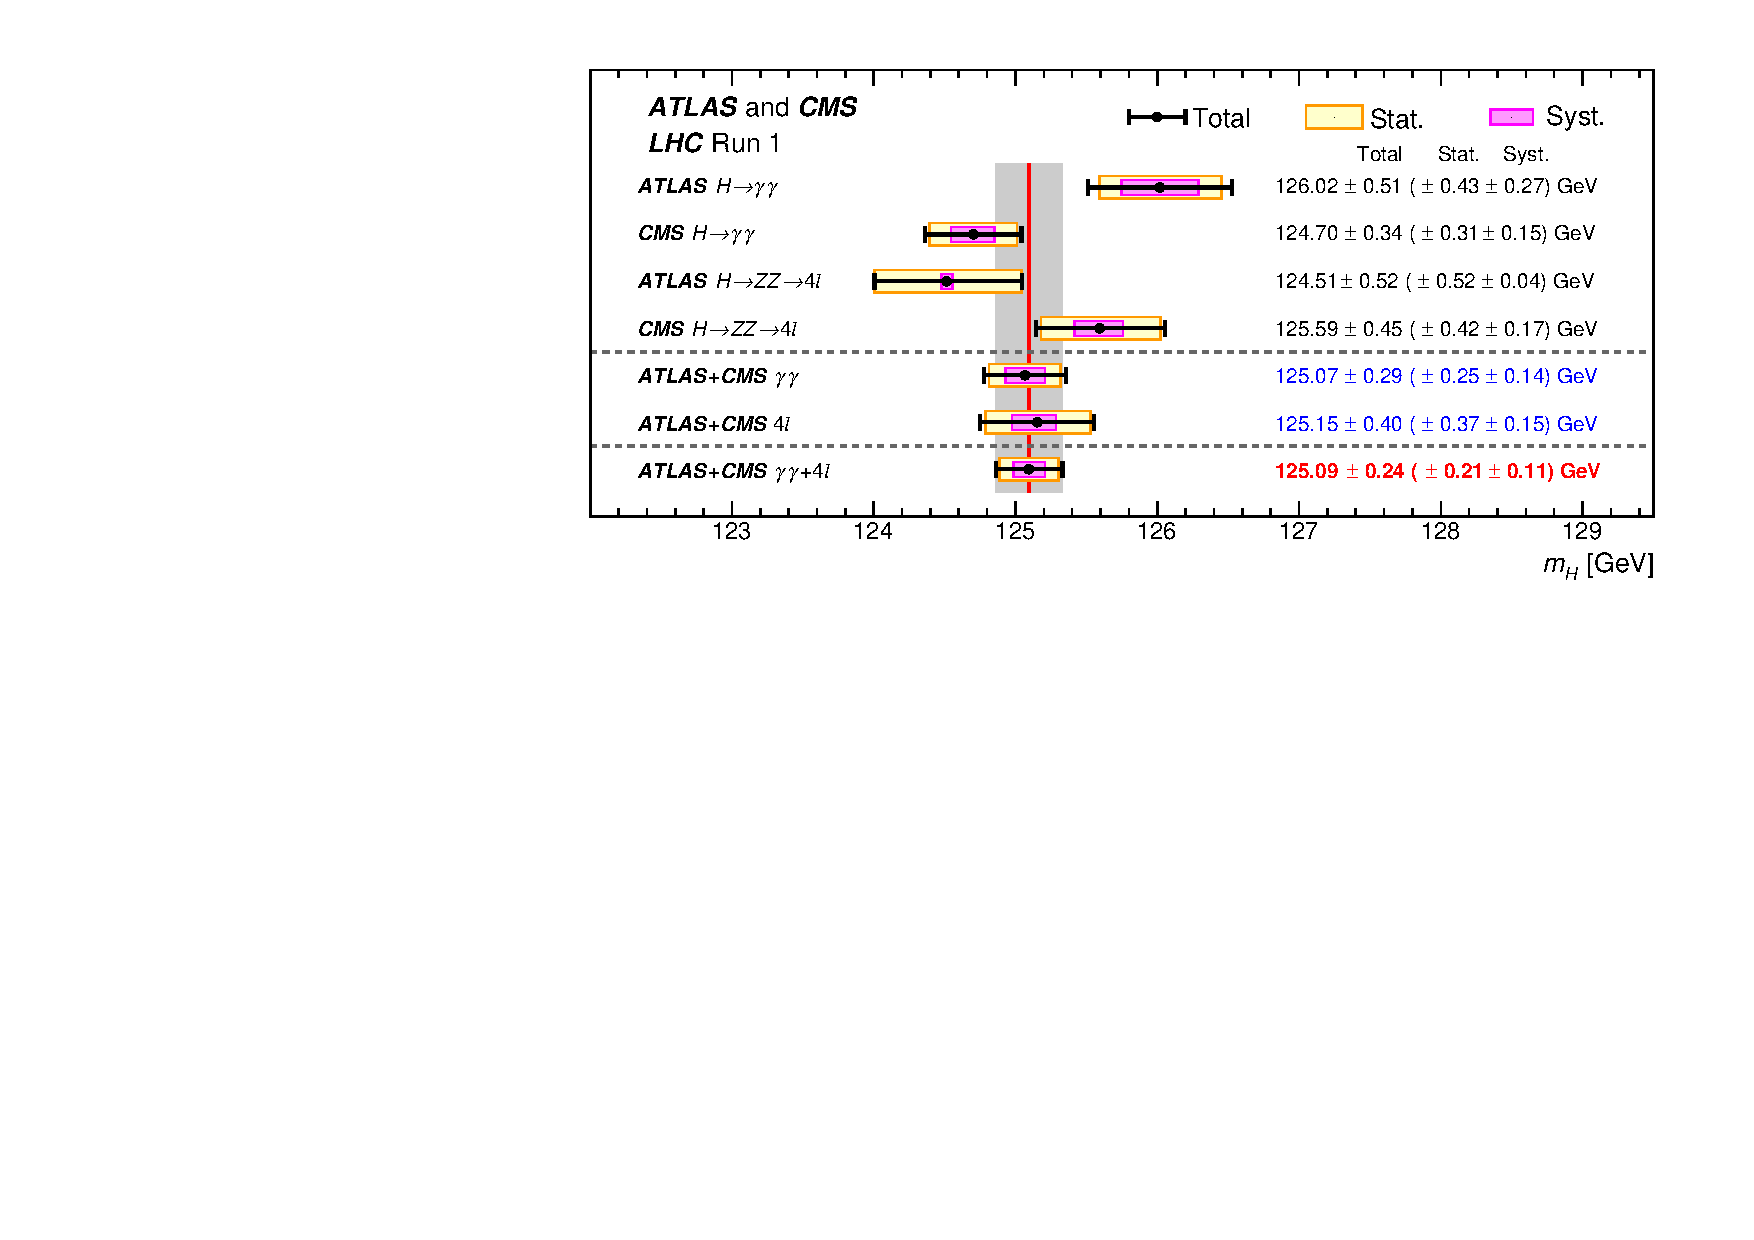
\includegraphics[width=0.8\textwidth]{figures/higgs_atlas_cms_mass}
  \caption{Resumen de las mediciones de la masa del bosón de Higgs de los
    distintos análisis de ATLAS y CMS, y del análisis combinado. Se indican las
    incertezas sistemáticas (bandas de color magenta), estadísticas (bandas de
    color amarillo), y total (líneas negras). La línea roja vertical y la
    correspondiente sombra gris indican el valor central y la incerteza total de
    la medida combinada, respectivamente\cite{HiggsMass_ATLAS_CMS}.}
  \label{fig:higgs_cms_atlas}
\end{figure}



\subsection{QCD y colisiones $pp$ en el LHC}
%% * From CERN-THESIS-2011-120.pdf y tincho

La cromodinámica cuántica (QCD) \cite{Ellis:1991qj} es la teoría de campos de gauge
renormalizable que describe la interacción fuerte entre las partículas que
poseen carga de color: \emph{quarks} y gluones. A diferencia de QED, los mediadores
de esta interacción, los gluones, poseen carga de color, por lo que
pueden interactuar entre ellos, dando lugar a un comportamiento inusual de la
interacción fuerte. La fuerza fuerte aumenta linealmente con la distancia entre
dos cargas. La constante de acoplamiento $\alpha_s$ depende entonces de
la distancia entre las cargas o de la escala de energía de la interacción. Se
dice que la constante ``corre'', siendo grande a bajas energía (o grandes
distancias) y haciéndose más chica a altas energías (o menores distancias).

El efecto neto de esta característica del acoplamiento fuerte es el
confinamiento, es decir, que las partículas con color no puedan existir
libremente. Solo estados de color neutro de múltiples partículas de color pueden
ser observados en la naturaleza viajando distancias macroscópicas. Los estados
que consisten en un par \emph{quark-antiquark} son denominados mesones y  los
 formados por tres \emph{quarks} son denominados bariones. El protón en un
barión constituido por dos \emph{quarks} $u$ y un \emph{quark} $d$, donde cada \emph{quark} tiene uno de
las tres posibles cargas de color para dejar un estado neutro. Estos tres \emph{quarks}
son llamados \emph{quarks} de valencia del protón, y están rodeados por un mar
de gluones y pares de \emph{quark-antiquark} que surgen de fluctuaciones cuánticas.
Otra consecuencia de la estructura de la interacción fuerte es que los cálculos
perturbativos no son posibles en el régimen de grandes valores de $\alpha_s$.

El LHC es un colisionador de protones, por lo tanto es esencial una precisa
descripción de la estructura del protón, ya que una colisión $pp$ a altas
energías es básicamente una colisión de dos constituyentes del mismo.
A altas energías es posible entonces aplicar el llamado <<modelo de
partones>>, en el cual los hadrones están compuestos por partículas puntuales.
Este modelo fue introducido por Feynman \cite{PhysRevLett.23.1415} y Bjorken
\cite{PhysRev.185.1975} a fines de los a\~nos 60, para interpretar los
resultados de los experimentos de dispersión inelástica profunda (DIS)
electrón-nucleón en SLAC. Esta descripción ha probado ser una buena aproximación
para las interacciones partón-partón de gran trasferencia de momento pero no es
apropiado para modelar la interacción a bajas energías. Los quarks de valencia y
los \emph{quarks} y \emph{antiquarks} del mar junto con los gluones son llamados
<<partones>> del protón. Cada partón lleva solo una fracción del momento y la
energía del protón. Para la medición de una sección eficaz de dispersión fuerte
que involucre \emph{quarks} y gluones en el estado inicial, es necesario conocer el
momento de las partículas incidentes. Como los partones solo llevan una fracción
del momento del protón, y están en interacción permanente entre ellos, el momento es
desconocido, por lo que la escala de energía $Q$ de las colisiones varía. Además,
como se mencionó, los \emph{quarks} ($q$) y
gluones ($g$) salientes no pueden observarse directamente debido al confinamiento,
pero son observados en el detector como \emph{jets}. Entonces no es posible
medir una sección eficaz partónica como $\sigma(qg \to qg)$, pero se puede hacer
una medida inclusiva, como la sección eficaz hadrónica $\sigma(pp \to jj)$ con
dos jets en el estado final. En teoría de perturbaciones, para pasar desde la
sección eficaz partónica a la sección eficaz hadrónica es necesario conocer la
probabilidad de que un partón de tipo $n$ sea encontrado con una fracción de
momento $x$, es decir, las funciones de distribución partónica (PDF). Estas
funciones son determinadas a partir de datos obtenidos de los propios
experimentos de altas energías, ya que no pueden determinarse a partir de la
teoría.

Esta conexión entre los hadrones observables y el nivel partónico es posible
gracias al concepto de <<factorización>>, que permite una separación
sistemática entre las interacciones de corta distancia (de los partones) y las
interacciones de larga distancia (responsables del confinamiento de color y la
formación de hadrones). El teorema de factorización \cite{Ellis1978281}
establece que la sección eficaz de producción de cualquier proceso de QCD del
tipo $A+B\to X$, siendo $a_i(b_j)$ los constituyentes del hadrón inicial $A(B)$,
puede ser expresada como:

\begin{equation}
  \sigma_{AB\to X} = \sum_{ij} \int dx_{a_i} \, dx_{b_j} \, f_{A/a_i} (x_{a_i}, \mu_F^2) \, f_{B/b_j} (x_{b_j}, \mu_F^2) \, \sigma_{a_i b_j\to X}(\mu_F^2,\mu_R^2)
\end{equation}
%
donde $x_i(x_j)$ es la fracción del momento del hadrón $A(B)$ que lleva el
partón $a_i(b_j)$ y $\sigma_{a_i b_j\to X}$ es la sección eficaz de la
interacción a nivel partónico, calculada a un dado orden de perturbaciones y una
escala de renormalización $\mu_R$. La escala de renormalización es introducida
para absorber las divergencias ultravioletas que aparecen en los cálculos
perturbativos más allá de LO. Las funciones $f_{h/n}(x_n,\mu_F^2)$ son las PDF,
que representan la probabilidad de encontrar un partón de tipo $n$ en el hadrón
$h$ con una fracción de momento $x_n$, dada una escala de factorización $\mu_F$.
Esta escala es un parámetro arbitrario introducido para tratar singularidades
que aparecen en el régimen no perturbativo. Estas divergencias son absorbidas,
en forma similar a la renormalización, dentro de las funciones de distribución
partónicas a la escala $\mu_F$. Si bien las PDF no pueden ser determinadas
perturbativamente, se puede predecir su dependencia con el impulso transferido $Q^2$
por medio de las
ecuaciones de evolución DGLAP \cite{Gribov:1972ri,Lipatov:1974qm,ALTARELLI1977298}.
De esta forma, la medida experimental de su
forma funcional a un dado $Q_0^2$ fijo permite obtener predicciones de las PDF
para un amplio espectro de $Q^2$.

A modo de ejemplo, en la \cref{fig:sm_atlas_xs}, se muestra el buen acuerdo
entre la sección eficaz de algunos procesos del SM medidas por ATLAS y las
predicciones teóricas. Las observaciones experimentales realizadas en LHC
resultan compatibles con el SM a un nivel de muy alta precisión.

\begin{figure}[!htb]
  \centering
  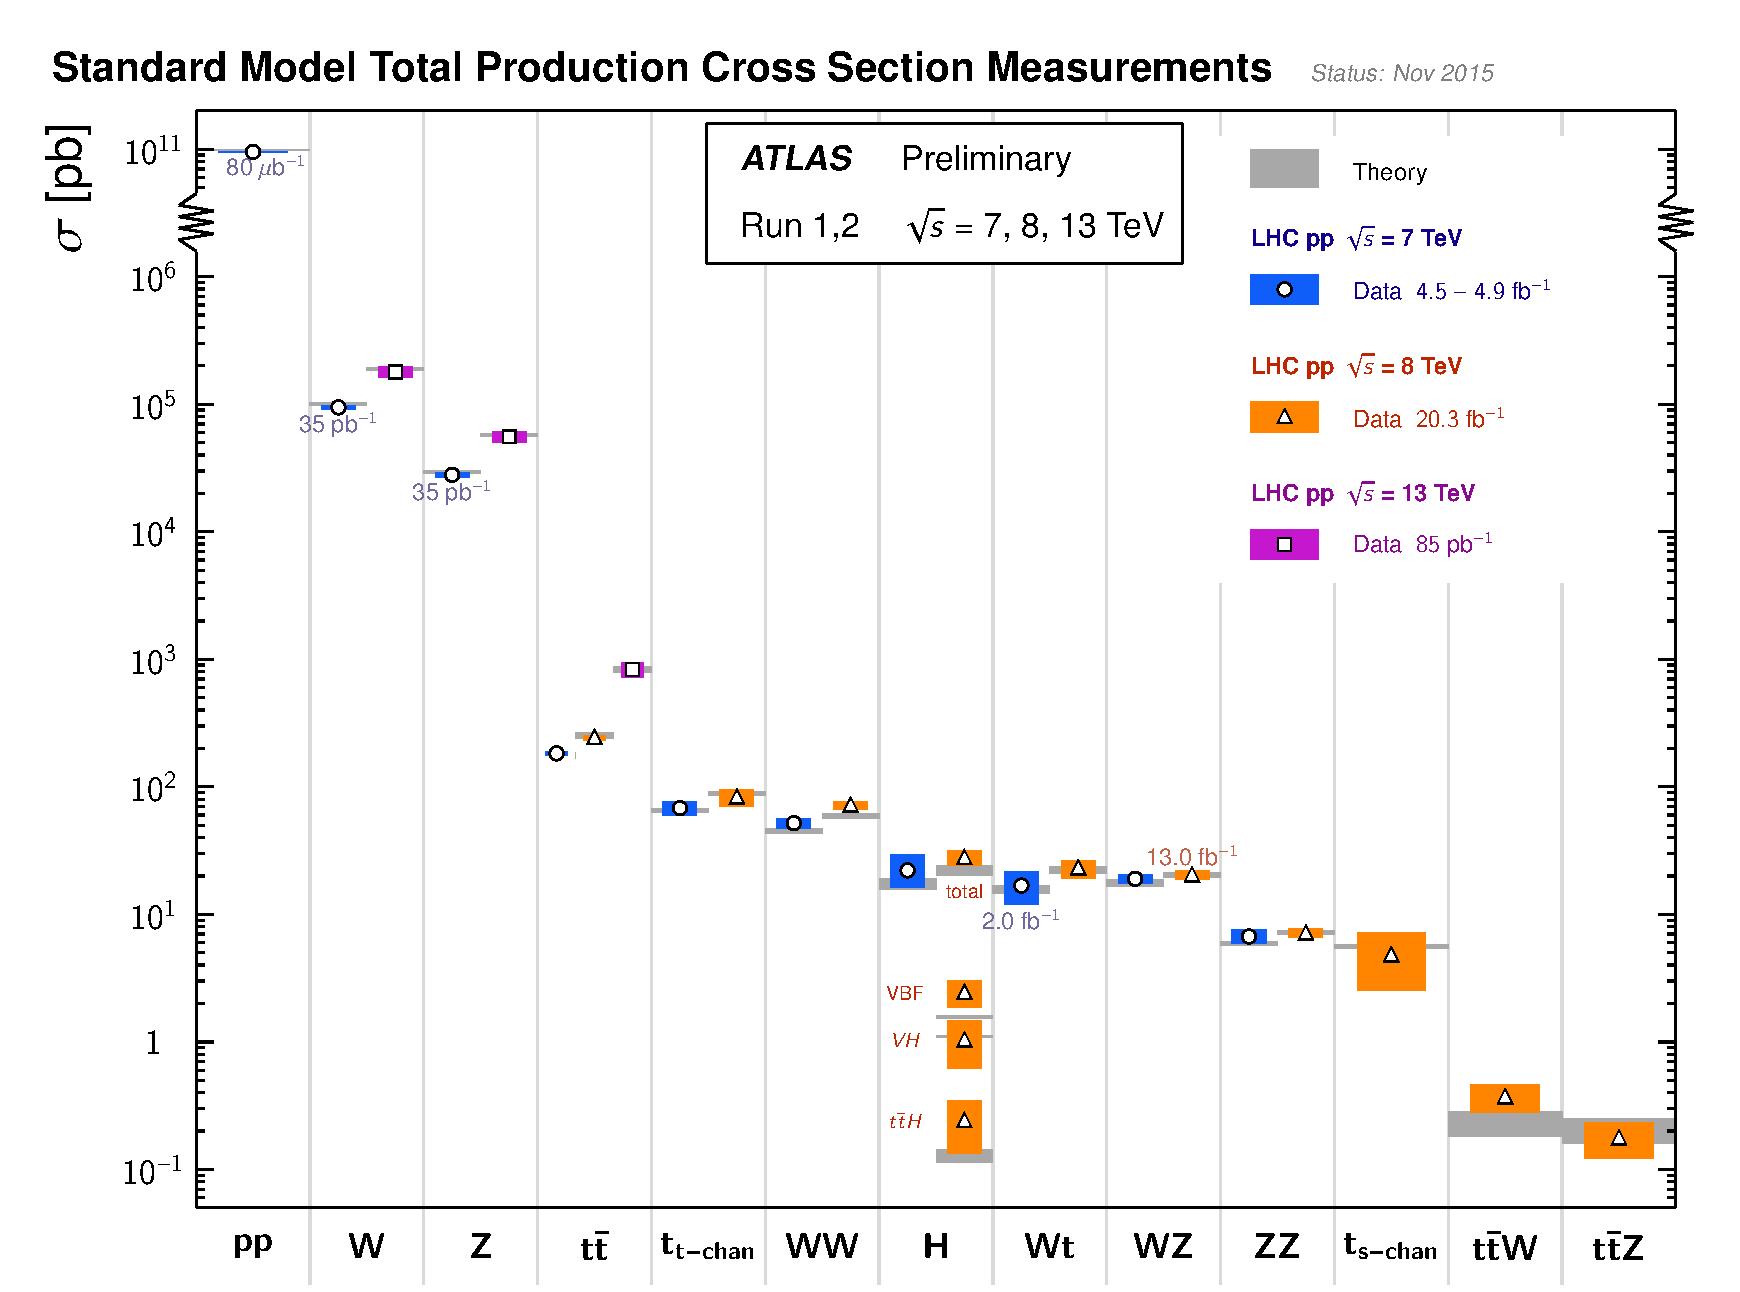
\includegraphics[width=1\textwidth]{figures/ATLAS_a_SMSummary_TotalXsect_new.pdf}
  \caption{Resumen de las distintas medidas de sección eficaz de producción de
    procesos del SM, comparadas con sus valores teóricos esperados.
    Los valores teóricos esperados fueron calculados como mínimo a NLO\cite{ATLASSM}.}
  \label{fig:sm_atlas_xs}
\end{figure}




\subsection{Física más allá del SM}

El SM provee una descripción notablemente exitosa de todos los fenómenos
accesibles con los experimentos de altas energías disponibles actualmente. Sin
embargo, también se sabe que el SM deja cuestiones sin resolver, tanto desde el
punto de vista teórico, como experimental.

El hecho de que existan cuatro tipos de interacciones distintas e independientes
es un poco insatisfactorio y desde Einstein se ha especulado que ellas sean
distintas manifestaciones de un único campo unificado. El descubrimiento de los
bosones $Z$ y $W$, tal como fueron predichos por la teoría electrodébil,
significaron un triunfo de la idea de una teoría unificada de las fuerzas. Cabe
destacarse que los resultados de las medidas de precisión de la sección eficaz
diferencial de las corrientes cargadas y neutras en la dispersión inelástica
profunda, obtenidos en HERA \cite{Hera}, proporcionaron una clara evidencia de
la unificación electrodébil.

Todo parece indicar que el SM es una teoría efectiva a bajas energías, muy
precisa hasta escalas de energía del orden de los 100 {\gev}. Sin embargo, los
físicos consideran que el éxito del SM no se extenderá a energías mayores. Esta
idea impulsa intentos de incorporar el SM en una teoría más fundamental. Incluso
ante la ausencia de la gran unificación de las fuerzas electrodébil y fuerte a
una escala muy alta de energía, el SM debería ser modificado para incorporar los
efectos de la gravedad a la escala de Planck.

Otro síntoma de incompletitud es la gran cantidad de parámetros libres que deben
ajustarse a los datos observados, ya que no resultan de principios teóricos más
fundamentales. El SM tiene 19 parámetros libres: 13 del sector de Yukawa, 2 del
sector de Higgs, las tres constantes de acoplamiento, y una fase del lagrangiano
de QCD.

En este contexto también resulta inexplicable por qué el cociente entre la escala
electrodébil y la escala de Planck $M_W/M_P \sim 10^{-17}$ es tan chico, lo que
se conoce como <<problema de jerarquía>>.
Por otro lado, en el SM, la escala de las interacciones electrodébiles se derivan de un
campo escalar elemental que adquiere un valor de expectación de vacío $v = 2
M_W /g = 246 \gev$. Sin embargo, si se acopla una teoría de partículas
escalares a nueva física a alguna escala arbitraria $\Lambda$, las correcciones
radiativas al cuadrado de la masa escalar son del orden de $\Lambda^2$, debido a
las divergencias cuadráticas en la autoenergía, lo cual indica la sensibilidad
cuadrática a la mayor escala de energía de la teoría. Por esto, la masa
``natural'' de cualquier partícula escalar es $\Lambda$. Así, para tener una teoría
electrodébil exitosa, la masa del Higgs debe ser del orden de la escala
electrodébil. Este hecho, que la masa del bosón de Higgs no puede ser igual a su
valor natural de $M_P$, es llamado <<problema de naturalidad>>.

Desde el punto de vista experimental, también existen algunos resultados que no
pueden acomodarse dentro del SM. El SM considera a los neutrinos como partículas
no masivas, pero distintos
experimentos\cite{PhysRevLett.101.111301,PhysRevD.78.032002} han observado que
los mismos presentan oscilaciones de sabor, lo que puede explicarse en el caso
en que estos tengan una masa no nula. Por el momento sólo existen límites
superiores para estas masas (ver \cref{tab:fermions}), que son muy peque\~nas
comparadas con las de los demás fermiones. El término de masa para fermiones
puede escribirse usando el doblete de Higgs si existen grados de libertad
asociados con los fermiones de quiralidad izquierda y derecha para un dado
sabor. La masa obtenida por esta interacción es llamada masa de Dirac. Para que
este mecanismo puede ser utilizado en los neutrinos, deberían existir los
neutrinos de quiralidad derecha.

El SM tampoco provee un candidato para explicar la naturaleza de la materia
oscura. La existencia de la materia oscura fue inferida por primera vez como
resultado de las inconsistencias observadas entre la masa estimada de las curvas
de rotación galácticas y de su luminosidad\cite{DM1}. Solo el 4\% del universo
consiste de la materia que conocemos\cite{DM2}, cerca del 73\% es
energía oscura, y el restante 23\% es materia oscura. La única partícula del SM
que podría ser un candidato viable de materia oscura es el neutrino, pero como
su masa es muy chica para poder explicar estos fenómenos, ha sido descartado.

Son varias las teorías que intentan explicar parcial o totalmente los problemas
mencionados anteriormente. Estas se conocen como teorías de física más allá del SM y entre
ellas se encuentra la Supersimetría, modelos con dimensiones extra, teoría de
cuerdas, teorías tecnicolor, etc. En la siguiente sección se explica brevemente
en qué consiste una de las teorías de física más allá del SM más motivadas desde
el punto de vista teórico, que es la Supersimetría.
